%!TEX root = report.tex

\chapter{Analysis} % (fold)
\label{cha:analysis}
The previous section described structural analysis and FEA in general and presented different software programs that can be used in the analysis. This section presents how FEA is performed at Andritz Hydro AB based on the investigation made by the author of this thesis. The investigation is the basis of the improvement suggestions that are given in sourcethis section.

\section{Analysis Workflow at Andritz} % (fold)
\label{sec:analysis_workflow_at_andritz}
% Product development process: FEA p. 12-13
The structural analysis begins with a CAD model created by the design team. The design engineers at Andritz Hydro AB use Siemens NX to create CAD models, internally in NX these models are called \textit{parts}. The parts are given a reference number to a database where they are stored, and this reference number is passed on to the calculation team. As described in Section~\ref{sub:pre_processing}, the CAD model needs to be cleaned of features that are unnecessary to the analysis. Since the cleaning process can change the model significantly it is not appreciated by the design engineers that the model they created is altered, therefore, a copy of this model is created which can be prepared for analysis. A copy is created by creating a new part in the database that is assigned to the calculation engineer and then using a synchronous modelling tool called \textit{WAVE Geometry Linker} to link the part created by the design engineer.

The cleaning process is done in NX with the synchronous modelling tools that is described in Section~\ref{sec:siemens_nx}. Depending on the level of detail of the model that is provided, the amount of work that is needed on the cleaning process can range from very little to a significant part of the entire analysis process. 

When the part is ready to be meshed it is exported from NX. There exists several formats to export a CAD model such that the details of the model are preserved, and at Andritz the STEP (standard for the exchange of product model data) format is used. A STEP file describes a CAD model according to an ISO standard which is used for file exchange~\cite{stepiso}.

The rest of the pre-processing is carried out in the Salomé Platform described in Section~\ref{sec:salom_platform}. The STEP file is imported and the Geometry module is selected. As described in Section~\ref{sub:geometry_module}, groups are created in the Geometry module to define where local mesh refinement is needed, where boundary conditions are applied and possible contact surfaces.

After the groups are defined the the analyst change to the Mesh module where the model is meshed. The meshing process in Salomé is described in Section~\ref{sub:mesh_module}. 3D models are usually meshed with tetrahedrons (see Sec.~\ref{sub:elements}) and 2D models are usually meshed with triangles, in both cases the NETGEN algorithm is used.

To solve the model Code Aster is used and, as is described in Section~\ref{sec:code_aster}, Code Aster requires the mesh to be described in a text file where patches, on which boundary conditions are applied, are defined. Therefore, mesh groups are defined in the Mesh module before the mesh is exported.

The final steps of the analysis (solution and post-processing) has not been investigated to the same level of detail, and are therefore summarised just to give a complete description of the analysis workflow. Given a file describing the mesh and a COMM file that describes the simulation, Code\_Aster can run the simulation. The COMM file describes the type of simulation, boundary conditions and other parameters depending on the type of simulation. The output of the simulation is the results that can be visualised and analysed with the ParaVis module.

The workflow described is presented in Figure~\ref{fig:andritz_workflow}. 

\begin{figure}[t]
	\begin{center}
		\begin{tikzpicture}[node distance=5mm]
			\node[rect] (design)					{Design};
			\node[rect] (clean)	[below=of design] 	{Model clean-up};
			\node[rect] (step)	[below=of clean]	{Export part as \texttt{.step} file};
			\node[rect] (salom)	[below=of step]		{Import to Salomé};
			\node[rect] (group) [below=of salom] 	{Create groups};
			\node[rect] (mesh)	[below=of group]	{Create mesh};
			\node[rect] (mail)	[below=of mesh]		{Export as \texttt{.mail} file};
			\node[rect] (comm)	[below=of mail]		{Write Code Aster input file};
			\node[rect] (solve)	[below=of comm]		{Solve};
			\node[rect] (vis)	[below=of solve]	{Visualise and analyse results};
			\path (design)	edge[->]	(clean)
				  (clean)	edge[->]	(step)
				  (step)	edge[->]	(salom)
				  (salom)	edge[->]	(group)
				  (group)	edge[->]	(mesh)
				  (mesh)	edge[->]	(mail)
				  (mail)	edge[->]	(comm)
				  (comm)	edge[->]	(solve)
				  (solve)	edge[->]	(vis);
			\draw [->] (vis.west) -- ++(-.5,0) |- (design.west);
		\end{tikzpicture}
	\end{center}
	\caption{Current analysis workflow at Andritz Hydro AB.}
	\label{fig:andritz_workflow}
\end{figure}

If the results are feasible the development of the CAD model can continue, and preparations for the manufacturing process can begin. However, if the results show that the model does not fulfil the requirements the model needs to be redesigned and the analysis repeated on the updated model. This iteration procedure is standard in product development. Since the analysis of the updated model is likely to be very similar to the original model some of the steps described in Figure~\ref{fig:andritz_workflow} are reusable, however, some steps have to be performed again. During the analysis of a redesigned model the following steps cannot be reused:
\begin{itemize}
	\item Model clean-up
	\item Create geometric groups
	\item Create mesh
	\item Create mesh groups
\end{itemize}
Obviously the visualisation and analysis of the results need to be repeated, but that is unavoidable. The four steps mentioned above are all part of the pre-process of the analysis, and they could be a very time consuming part of the analysis, so it would be favourable to find a solution that could reuse the fact that these steps already have been performed on a very similar model. 

It is also possible that half way through the analysis there could be an update to the original CAD model that is independent of the analysis. If the update is significant to the analysis a new analysis needs to be started in this case as well. This is because the link between the CAD model and the analysis model is broken during the first step when the CAD model is copied. This is obviously very frustrating and time consuming for the analyst. Since these updates of the CAD model are impossible to prevent a solution that diminish the effect of the update is very desirable.
% subsection analysis_workflow_at_andritz (end)

\section{Using NX Advanced Simulation} % (fold)
\label{sec:using_nx_advanced_simulation}
The previous section described the structural analysis workflow at Andritz Hydro AB and highlighting parts of the workflow that is inefficient, especially if a new iteration is started. This section describes a possible solution to some of the problems that are discussed. NX Advanced Simulation (described in Sec.~\ref{sec:siemens_nx}) supports the entire FEA process 

Suggested workflow with NX Advanced Simulation:

\begin{figure}[t]
	\begin{center}
		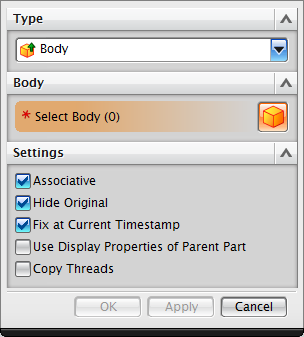
\includegraphics{WAVEGeometryLinker}
	\end{center}
	\caption{WAVE Geometry Linker dialogue box in NX.}
	\label{fig:WAVEGeometryLinker}
\end{figure}
% subsection using_nx_advanced_simulation (end)

\section{Salomé API Script} % (fold)
\label{sec:salom_api_script}
Salomé provides a Python API for every module that allows the user to write Python scripts to automate processes that are often repeated. As is described in Section~\ref{sec:analysis_workflow_at_andritz}, there are steps in the pre-process of the FEA workflow that can be time consuming to perform manually, and it is especially inefficient if a new iteration is started since the steps that already have been done, must be repeated. This section presents a solution that efficiently automate some parts of the pre-processing steps and at the same time reduces the amount of work that have to be repeated if a new iteration is started.

The main issue with the workflow in Figure~\ref{fig:andritz_workflow} is that the connection between the CAD model and the FE model is lost when the part is exported from NX and imported to Salomé. All the steps of the pre-processing that is done in Salomé needs to be repeated with the current workflow. Therefore, it would be better to move as many of the steps as possible from Salomé to NX, since these steps would not have to be repeated. Within the current NX license at Andritz Hydro AB, the step that can be moved is the definition of the groups.

The main idea of the new workflow is to clean the model and define the groups in NX, and when the model is exported the group definitions are included in the STEP file. In Salomé the model is imported and the groups defined in NX are automatically created. The model is meshed and the groups that should be included in the text file describing the mesh are automatically created in the Mesh module.

\subsubsection{Defining Groups in NX} % (fold)
\label{ssub:defining_groups_in_nx}
In NX any geometrical object (solid, face, edge, etc.) or collection of objects can be given a name. The name and which geometrical object it is associated with are included in the STEP file when the model is exported. The import utility in Salomé does not recognise these names as groups when the STEP file is imported, therefore these names needs to be manually translated to group objects. The Geometry API provides several functions to automate this process, and the solution is a function named \texttt{CreateGroups} which is presented in Appendix~\ref{sec:creategroups}. \texttt{CreateGroups} creates the groups that are defined in NX of the object that is selected in the object browser.

The \textit{Explode} function creates sub-shapes of a specified type of an object, for example if a box is exploded to faces all eight faces of the box are created. Using this function the groups defined in NX can be recreated.

See example in Figure~\ref{fig:example1}.

\begin{figure}[t]
	
\begin{subfigure}{.3\textwidth}
	\begin{center}
		\includegraphics{Untitled}
	\end{center}
	\caption{Object browser}
	\label{fig:objbrow}
\end{subfigure}
\begin{subfigure}{.7\textwidth}
	\begin{center}
		\includegraphics[trim=10 80 50 0,clip,scale=.5]{example.png}
	\end{center}
	\caption{A simple example.}
	\label{fig:example1}
\end{subfigure}

	\caption{Caption here}
	\label{fig:figure1}
\end{figure}


% subsubsection defining_groups_in_nx (end)

% The proposed workflow is presented in Figure~\ref{fig:script_workflow}.

% \begin{figure}[t]
% 	\begin{center}
% 		\begin{tikzpicture}[node distance=5mm]
% 			\node[rect] (design)					{Design};
% 			\node[rect] (clean)	[below=of design] 	{Model clean-up};
% 			\node[rect] (group) [below=of salom] 	{Create groups};
% 			\node[rect] (step)	[below=of clean]	{Export part as \texttt{.step} file};
% 			\node[rect] (salom)	[below=of step]		{Import to Salomé};
% 			\node[rect] (mesh)	[below=of group]	{Create mesh};
% 			\node[rect] (mail)	[below=of mesh]		{Export as \texttt{.mail} file};
% 			\node[rect] (comm)	[below=of mail]		{Write Code Aster input file};
% 			\node[rect] (solve)	[below=of comm]		{Solve};
% 			\node[rect] (vis)	[below=of solve]	{Visualise and analyse results};
% 			\path (design)	edge[->]	(clean)
% 				  (clean)	edge[->]	(step)
% 				  (step)	edge[->]	(salom)
% 				  (salom)	edge[->]	(group)
% 				  (group)	edge[->]	(mesh)
% 				  (mesh)	edge[->]	(mail)
% 				  (mail)	edge[->]	(comm)
% 				  (comm)	edge[->]	(solve)
% 				  (solve)	edge[->]	(vis);
% 			\draw [->] (vis.west) -- ++(-.5,0) |- (design.west);
% 		\end{tikzpicture}
% 	\end{center}
% 	\caption{Current analysis workflow at Andritz Hydro AB.}
% 	\label{fig:script_workflow}
% \end{figure}
% subsection salom_api_script (end)




% section analysis (end)